\paragraph{Image acquisition process details} 
    The cells used in this research are growing in 96-well plates. A plate or a microplate in biology is a flat plate with multiple wells. The microscope used in the experiments takes several photos of each well plate in random locations within it. The reason for that lies in the focusing settings of a  microscope. To get a reasonably good, and not blurry, photo, a microscope has to focus on a specific location of the plate. In the microscope used for this research the choice of this location happens automatically. It is not possible to choose which region of a well-plate will be photographed, therefore it is also not possible to do consecutive images without intersections as the regions are chosen randomly (see Figure \ref{fig:random-dic}). 
    
    It might be problematic in the following sense: photos taken in such a manner do not guarantee that the focus will land in distinct spots all the time. Meaning that some cells present in one of the photos might appear in the other ones as well. Since the photos are high-resolution they will first be split into crops of size $256 \times 256$ each during the preprocessing. It might happen that the same cells appear in several crops. That is why after the split of the image data between train, test and validation sets it might also happen that the same set of cells will once land in the train set and another time in the validation set, which will lead to a not completely fair and representative validaiton metrics during training.
    
    In order to overcome this problem much more expensive equipment is needed. Since it does not cause fundamental problems in this case, except for the fact that the validation metrics might be lower than what they should have been, we neglect this effect for the remainder of the work. 
    
    \begin{figure}[htb]
        \begin{center}
            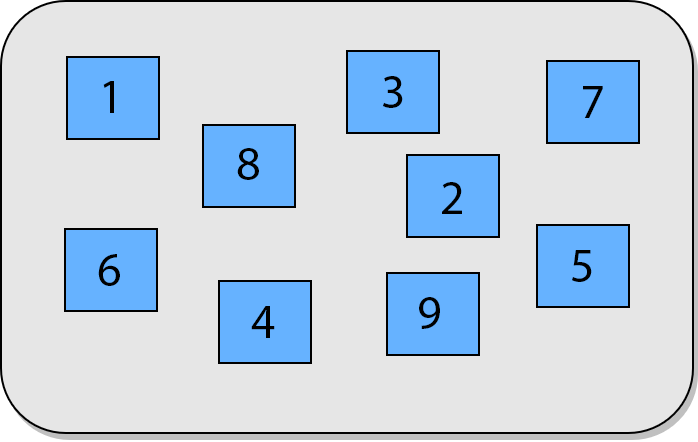
\includegraphics[width=0.3\linewidth]{bilder/dic-random.png}
            \caption{Radom location of the microscope focus for one well-plate}\label{fig:random-dic}
        \end{center}
    \end{figure}